\documentclass[10pt,a4paper]{article}
\usepackage[margin=0.55in]{geometry}
\usepackage[T1]{fontenc}
\usepackage{lmodern}
\usepackage{booktabs,array,tabularx,amsmath,enumitem,xcolor,tikz,hyperref,titlesec,microtype}
\usetikzlibrary{positioning}
\newcolumntype{P}[1]{>{\raggedright\arraybackslash}p{#1}}
\hypersetup{colorlinks=true,linkcolor=black,urlcolor=blue}
\setlist{nosep,leftmargin=*}
\titleformat{\section}{\large\bfseries}{\thesection}{0.6em}{}
\titleformat{\subsection}{\normalsize\bfseries}{\thesubsection}{0.5em}{}
\titlespacing*{\section}{0pt}{8pt}{3pt}
\titlespacing*{\subsection}{0pt}{5pt}{2pt}
\renewcommand{\arraystretch}{1.10}
\emergencystretch=2em
\sloppy
\setlength{\tabcolsep}{2pt}
\setlength{\parskip}{2pt}
\setlength{\parindent}{0pt}
\pagestyle{plain}

\begin{document}

{\LARGE\bfseries Reducing Avoidable Steel Loss: a Measure-First Pilot}\\[2pt]
{\large Forward Deployed Engineer case study --- Client B, Structural Steel}\\[2pt]
\small Prepared by Krushna Raut \quad|\quad October 2026 \quad|\quad Confidential: based on client discovery calls 1--2

\vspace{4pt}
\noindent\fbox{\parbox{\dimexpr\textwidth-2\fboxsep-2\fboxrule\relax}{\small
\textbf{In short.} The client asked for ``AI for nesting''. What they lack is a trustworthy measurement of where steel is lost, how much of it may be preventable, and whether existing Strumis auto-nesting performs worse than manual nesting. I recommend a \textbf{staged, 6-week ``Measure and Prove'' pilot}. The committed core is (1) a reconciled material baseline and (2) a controlled comparison of manual nesting with configured Strumis auto-nesting. A read-only offcut-matching proof of concept is conditional on data readiness. The first result is a provisional baseline by week 3. No custom AI nester or automated cross-project transfer is built unless evidence and client policy justify it. The INR 18 lakh price below is an illustrative estimate, not a validated quote.}}

%==================================================================
\section{Problem understanding}
\subsection{What they asked for vs.\ what they need}
\begin{tabular}{@{}P{3.6cm}P{6.2cm}P{6.2cm}@{}}
\toprule
 & \textbf{Asked for} & \textbf{Needed} \\
\midrule
Goal & AI to optimise nesting and reduce waste (plate 20--25\%, profiles 5--10\%, overall 7--10\%). & A defensible number: how much steel is lost, where, and how much of it was \emph{preventable}. \\
Method & ``AI for nesting'', plus auto-allocation of material between projects. & Evidence on three separate problems: \textbf{cutting} (can the same parts use less plate?), \textbf{offcut reuse} (are usable leftovers missed?), \textbf{accounting} (may material move between projects, and at what cost?). \\
Starting point & Nesting, ``If I have to pick one''. & Nesting is a reasonable anchor, but it is only valid after a baseline; the other four areas are unmeasured and should be ranked by data readiness. \\
\bottomrule
\end{tabular}

\subsection{Stakeholders}
The contact (Cost Control) states he/she ``doesn't know much about nesting''; the nesting, engineering and yard teams were not on either call. Everything about their priorities below is \emph{inferred}, and the first action is to meet them.

\begin{tabular}{@{}P{3.3cm}P{6.4cm}P{6.3cm}@{}}
\toprule
\textbf{Who} & \textbf{What they want} & \textbf{What I need to tell / get from them} \\
\midrule
Cost Control contact (sponsor) & A number and a business case for management; a quick update ``within this week''. & A forwardable note; a baseline in 3 weeks; he/she brings Finance and nesting to the next call. \\
Nesting lead and planners & Control of the cutting plan; good usable offcuts; no unfair blame if auto-nesting loses. & The tool assists and they approve every plan; the bake-off is scored blind by them against criteria agreed in advance. \\
Finance / project accounting & Costs stay loaded to the owning project; clean audit trail. & No material transfer until they set a rule (price, credit, approval); we ask for a rule, not a system change. \\
Engineering / drawing office & Accurate drawings; fewer disputes over revisions; recoverable losses. & A sample of revision history; identify client-caused revisions that may be claimable and internal-error losses. \\
Yard and stores & Find the right plate without moving others. & Only the offcut location convention for now; yard optimisation is later. \\
Planning, procurement, factory ops & Delivery dates met; CNC throughput protected. & Plans must pass machine and schedule checks; nothing changes on the shop floor in the pilot. \\
Management & Stop hiring extra trailers; visible return; low risk. & Fixed fee, stage gates, a stop rule. \\
\bottomrule
\end{tabular}

\subsection{As-is process (as I understand it)}
\small
Bid $\to$ Estimate $\to$ Plan and buy (per project, early if delivery is early) $\to$ Engineering releases drawings (revisions follow) $\to$ \textbf{Nesting} (manual, in Strumis/PLM) $\to$ Sizing (CNC cutting) $\to$ Fabrication $\to$ Coating $\to$ Dispatch (13 own trailers, extra hired). Strumis acts as their ERP.
\normalsize

Observed pain points, with source:
\begin{itemize}
\item \textbf{P1 No loss data:} cannot say how much is wasted, how much is preventable, or which stock sits unused (call 1).
\item \textbf{P2 Manual vs.\ auto unproven:} the nesting team says auto wastes more; the contact says he/she ``is not sure how accurate that is'' (call 2). This is second-hand.
\item \textbf{P3 Per-project material:} each project has its own purchases and rates; the contact is unsure if one plate can be shared across projects (call 2).
\item \textbf{P4 Offcuts:} recorded and checked first, but ``could be done better'' (call 2, opinion, not measured).
\item \textbf{P5 Revisions:} no clear record; losses from client revisions are claimable, but own-error losses are unknown (call 2).
\item \textbf{P6 Yard:} no storage sequence; needed plates end up at the bottom; demand shifting with projects on hold (call 2).
\item \textbf{P7 Equipment:} CarTrack and a booking system installed 6 months ago, barely analysed, yet trailers are still hired (call 2).
\end{itemize}

%==================================================================
\section{What I don't know yet (ranked)}
Ranked by how much the answer would change the recommendation. We meet the nesting lead, a Finance contact and engineering on call 3.

\small
\begin{tabular}{@{}cP{4.6cm}P{5.4cm}P{4.9cm}@{}}
\toprule
\# & \textbf{Question (ask whom)} & \textbf{Why it changes the plan} & \textbf{Assumed until answered} \\
\midrule
1 & Can Strumis export, read-only, per-plate nesting reports (plate, grade, thickness, parts, utilisation) and the offcut register for the last 12 months? (IT, nesting lead) & Without data, the baseline and bake-off cannot run; this is the go/no-go gate in week 2. & Yes, in CSV or via a reporting view; about 60\% of plates are usable (complete). \\
2 & Why does the nesting team believe manual beats auto? Which rules do they apply (grade, weld prep, assembly grouping, remnant keeping, CNC limits), and was auto ever tuned? (nesting lead) & If auto lacks these rules, ``worse'' means ``not configured''. That decides whether to tune, to buy, or (unlikely) to build. & Auto was run with default parameters; part of manual's edge is unwritten rules we can encode. \\
3 & May an offcut from Project A be used on Project B, and at what cost credit? Who approves? Is it contractual or only policy? (Finance) & It decides whether cross-project matching is just a report or a real feature. & Not allowed without approval; same-project reuse is allowed; no transfer price is assumed. \\
4 & How are the 20--25\%, 5--10\% and 7--10\% computed (denominator, offcuts counted as waste?), and what share of tonnage is plate? (Cost Control) & The baseline and any savings claim depend on the definition; the three figures reconcile only if plate is about 13--33\% of tonnage (Appendix B). & Waste $=$ purchased weight $-$ part weight; offcuts returned to stock are counted separately; plate is about 20\% of tonnage. \\
5 & How are drawing revisions logged, and what tonnage was cut under a superseded revision last year? What is claimable? (engineering, Cost Control) & Claimable losses could be the fastest cash return, and revisions inflate the apparent nesting waste. & Revisions exist in Strumis/PLM only as unstructured history; treated as Phase 2, not in the pilot. \\
6 & What does ``a fixed budget at the start that they have to meet'' mean? Is there a per-project material allowance? (Cost Control) & A fixed allowance can discourage reporting offcuts or waste, and so distort the data we rely on. & There is a per-project allowance; offcut reporting may be incomplete. \\
7 & Can we get CarTrack and booking-system exports (6 months)? (Cost Control, IT) & It lets us choose the second area on evidence, at almost no cost. & Exports are available; trailer idle time is partly a booking-behaviour problem, not a fleet-size one. \\
8 & Are volumes typical right now? Projects are on hold. (planning) & A bake-off on unusual jobs may not generalise. & Historic jobs from the last 12 months give a fairer sample than the current queue. \\
\bottomrule
\end{tabular}
\normalsize

%==================================================================
\section{Solution}
\subsection{Options considered}
\small
\begin{tabular}{@{}P{4.1cm}P{6.0cm}P{5.7cm}@{}}
\toprule
\textbf{Option} & \textbf{What it is} & \textbf{Verdict} \\
\midrule
A. Reporting only & Spreadsheets of waste by project. & Needed, but does not test manual vs.\ auto; folded into the pilot. \\
B. Test and tune Strumis auto-nesting & Blind bake-off, same plates, manual vs.\ auto (configured with the team's rules). & \textbf{Included.} Cheapest way to test the central claim; may remove the need for any new software. \\
C. Offcut registry audit and matcher & Match registered offcuts to open part demands; suggestions only. & \textbf{Included, shadow mode.} Addresses ``unused material'' without touching accounting. \\
D. Custom AI / reinforcement-learning nester & Build our own optimiser. & \textbf{Rejected for now.} No evidence that it is needed; it would have to beat software we have not yet tested. Revisit only if the bake-off shows both manual and auto leave a large gap. \\
E. Buy a commercial nesting package & Another vendor's advice (the first supplier suggested packages). & \textbf{Deferred.} Only if auto cannot be tuned to match manual; the bake-off result becomes the buying spec. \\
F. Start with trailers or yard & Scheduling and layout analysis. & \textbf{Not first.} Trailer data exists, so a one-week look is added to select the second area; yard planning is unstable while projects are on hold. \\
G. Automatic cross-project allocation & Software moves material between projects. & \textbf{Rejected until Finance defines the rule.} A physically valid reuse is not necessarily financially valid. \\
\bottomrule
\end{tabular}
\normalsize

\subsection{Recommendation: ``Measure and Prove'' pilot (B + C + baseline)}
It is the best fit because (i) it uses what they already own (Strumis, offcut register); (ii) every claim the client made is either confirmed or refuted with their own data; (iii) the first output (baseline) arrives in 3 weeks, before any big spend; (iv) the nesting team is a participant, not a target; and (v) it tells us which of the four paths (tune, buy, offcut tracking, build) deserves Phase 2 money.

\subsection{What I would deliberately not build}
A custom deep-learning nester (the existing Strumis auto-nesting feature has not yet been fairly tested); automatic cross-project allocation (Finance has not defined ownership or cost-transfer rules); a yard digital twin (projects are on hold and the storage pattern may change when demand resumes); a new trailer/booking system (CarTrack and a booking system already exist but are under-analysed); write-back into Strumis (data quality and permissions are unverified); or any CNC plan change without nesting-lead approval.

\subsection{The other areas: how they get handled}
\begin{tabular}{@{}P{3.4cm}P{6.6cm}P{5.9cm}@{}}
\toprule
\textbf{Area} & \textbf{Next step} & \textbf{When} \\
\midrule
Drawing revisions & Create a structured revision log; link each revision to affected drawings, parts and plates; separate client-caused changes from internal errors; quantify potentially claimable tonnage and evidence gaps. & Assess early after the baseline: client-caused revisions may offer a nearer-term recovery opportunity, but no amount is assumed until records and contract terms are checked. \\
Trailer / equipment use & Analyse CarTrack and booking data: idle by asset, hire triggers, booking lead-times. & One-week data look in the pilot (week 1--2); decision at week 6. \\
Yard storage / loading plan & Sequence and location rules; load building by weight, size and delivery order. & Later; requires stable demand and the offcut location convention. \\
\bottomrule
\end{tabular}

%==================================================================
\section{Solution engineering}
\begin{center}
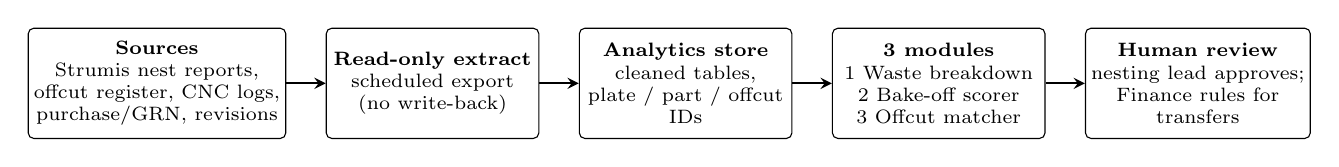
\begin{tikzpicture}[node distance=5mm,
 box/.style={draw, rounded corners=2pt, align=center, font=\scriptsize, minimum height=14mm, minimum width=27mm, inner sep=2pt},
 arr/.style={->, >=stealth, thick}]
\node[box] (a) {\textbf{Sources}\\Strumis nest reports,\\offcut register, CNC logs,\\purchase/GRN, revisions};
\node[box, right=of a] (b) {\textbf{Read-only extract}\\scheduled export\\(no write-back)};
\node[box, right=of b] (c) {\textbf{Analytics store}\\cleaned tables,\\plate / part / offcut\\IDs};
\node[box, right=of c] (d) {\textbf{3 modules}\\1 Waste breakdown\\2 Bake-off scorer\\3 Offcut matcher};
\node[box, right=of d] (e) {\textbf{Human review}\\nesting lead approves;\\Finance rules for\\transfers};
\draw[arr] (a)--(b); \draw[arr] (b)--(c); \draw[arr] (c)--(d); \draw[arr] (d)--(e);
\end{tikzpicture}
\end{center}

\subsection{Inputs and data}
\small
\begin{tabular}{@{}P{4.4cm}P{3.8cm}P{4.2cm}P{3.1cm}@{}}
\toprule
\textbf{Data} & \textbf{Source} & \textbf{Used for} & \textbf{Status} \\
\midrule
Plate nest reports (plate ID, grade, thickness, size, parts, utilisation) & Strumis nesting module & Baseline, bake-off & Assumed exportable (Q1) \\
Part lists / drawing revision per part & Strumis and/or PLM & Bake-off inputs; revision losses & System of record to confirm; migration may be incomplete \\
Offcut register (size, grade, location, project) & Strumis & Matcher & Exists; quality unknown \\
Actual cut logs, cut time & CNC controller & Cross-check planned vs.\ real & To be confirmed \\
Purchase, receipt, scrap weight & ERP, weighbridge & Mass balance & To be confirmed \\
Trailer / equipment data & CarTrack, booking system & Second-area selection & Exists \\
\bottomrule
\end{tabular}
\normalsize

\subsection{Logic}
\textbf{(1) Waste breakdown (mass balance per plate).}
\[
W_{\text{plate}} = W_{\text{parts}} + W_{\text{kerf/skeleton/trim}} + W_{\text{offcut, usable}} + W_{\text{offcut, scrap}} + W_{\text{revision}} + W_{\text{unexplained}}
\]
\textbf{Report categories separately; do not add overlapping categories into a single preventable-loss total.} For each plate, reconcile input weight against finished-part weight, measured scrap/kerf where available, identified reusable offcuts, and an unexplained balance. Report (a) finished-part yield, (b) scrap/trim rate, (c) reusable offcut inventory by weight and traceability, and (d) actual subsequent offcut reuse. An offcut is only a candidate for reuse when size, grade, thickness, certification and location are recorded; being labelled reusable is not itself a realized saving. Estimate the nesting opportunity as the paired difference between feasible manual and configured-auto plans on equivalent inputs. Track revision-related loss separately and only where revision records support attribution. Any remaining balance is reported as unexplained, not assigned to a cause.

\textbf{(2) Bake-off scorer.} The same part lists are nested manually (existing plans) and by Strumis auto-nesting configured with the team's rules; results are anonymised (A/B) before the nesting lead checks feasibility; yield, feasibility pass/fail and planner time are scored.

\textbf{(3) Offcut matcher (rules plus geometry, no ML needed).} Hard filters: grade, thickness, certification, minimum size, location. Then a geometric fit test (bounding box first, true outline next), ranked by fresh-steel weight avoided. Output: ``Offcut O-123 from Project A fits part P-45 of Project B, saves 38 kg, in Yard bay 4.'' It shows a suggestion only; a same-project match is a normal suggestion, a cross-project match is flagged ``needs Finance rule''.

\subsection{Sign-off and routine}
The nesting lead approves any plan, suggestion or change to the minimum-usable-offcut rule. Finance approves any cost-transfer rule. Engineering confirms the revision status for any affected part. In daily use, the matcher's list is a 10-minute review in the nesting team's morning routine; nothing is sent to CNC automatically. Hosting: a small virtual machine or on-premises server with read-only access; no client data leaves their environment unless they approve.

%==================================================================
\section{Evaluation}
\small
\begin{tabular}{@{}P{3.0cm}P{12.9cm}@{}}
\toprule
\textbf{Item} & \textbf{Definition} \\
\midrule
Primary metrics & Paired difference in finished-part yield by input weight for feasible plans using identical part lists. Secondary: scrap/trim rate, reusable offcut tonnes, actual reuse, feasibility pass rate, and planner minutes per plate. \\
Baseline & Target sample: up to 60 recent plates, stratified by grade/thickness and checked against available purchase, cutting and scrap records. This is a provisional baseline; coverage and reconciliation gaps will be stated explicitly. Cost Control signs off the definitions before results are treated as a business baseline. \\
Bake-off protocol & Target sample: 40 comparable historical plate-jobs, if data and operator time permit, sampled across grade/thickness and job complexity. Compare existing manual plans with Strumis auto-nesting configured using rules agreed with the nesting lead. Blind A/B review checks feasibility before yield and time are compared. Report paired differences and confidence intervals where sample size and data quality support them. Recalculate uncertainty from observed variability; 40 jobs is a practical pilot target, not a guarantee of statistical power. \\
Decision rules & Agree practical non-inferiority and time-saving thresholds with the client before examining results; the one-point yield and 30\% time-saving figures may be proposed for discussion, not treated as validated targets. If configured auto is acceptably close to manual and saves meaningful planner time without feasibility failures, consider it as a human-reviewed first draft. If manual performs better, retain it while diagnosing configuration and rule gaps. Consider buying/building only if a repeatable, economically material gap remains. \\
Offcut matcher test & Conditional on sufficiently complete offcut and demand data: replay up to 3 months of historical demand. Report candidate matches, engineering acceptance, traceability completeness, estimated fresh steel avoided, and matches actually consumed if records allow. Agree an acceptance target with the nesting lead before the test; separate same-project and cross-project matches. A suggested match is not counted as a realized saving. \\
Who measures & Our analyst runs the numbers; the nesting lead scores feasibility; Cost Control signs off the baseline definition. \\
\textbf{Stop / redirect} & If data access or quality is insufficient by the end of week 2, pause analytics and agree a manual-sampling fallback or stop. If no material, addressable opportunity is evidenced, do not proceed to implementation; compare validated opportunity value with implementation cost and the client's hurdle rate. If feasible plans cannot be evaluated consistently, revise the protocol before drawing conclusions. If Finance blocks cross-project transfers, exclude them from the value case; continue only if same-project reuse or the nesting comparison independently justifies further work. \\
\bottomrule
\end{tabular}
\normalsize

%==================================================================
\section{Build plan and timeline}
\small
\begin{tabular}{@{}P{1.6cm}P{5.5cm}P{4.3cm}P{4.5cm}@{}}
\toprule
\textbf{Week} & \textbf{Activities} & \textbf{Milestone} & \textbf{Depends on client} \\
\midrule
0 & Kickoff, NDA, access request. & Plan agreed. & Named nesting lead, IT contact, Finance contact. \\
1--2 & Shadow nesting; validate read-only extracts; agree definitions; brief scan of trailer/booking data only if readily available. & \textbf{Go/no-go gate (end wk 2)}. & Named owners, sample exports, and access to relevant records. \\
3 & Waste breakdown on 60 plates. & \textbf{First result:} baseline report. & Cost Control confirms definition. \\
3--5 & Bake-off: configure auto, run 40 plate-jobs, blind scoring. & Bake-off results. & Nesting lead: about 4 h/week; auto-nesting configuration help. \\
4--6 & Conditional, limited offcut-matching proof of concept in shadow mode; no integration or write-back. & Candidate-match report and data-quality findings. & Usable offcut register and demand data; Finance clarifies transfer constraints. \\
6 & Readout and decision. & Recommendation: tune / buy / build / stop; second area. & Management decision on Phase 2. \\
\bottomrule
\end{tabular}
\normalsize

\textbf{Indicative Phase 2} (not committed; scoped after week 6): 10--12 weeks to implement what the evidence supports, for example tuned auto-nesting as a first draft, the offcut matcher in daily use, revision tracking, or a trailer-utilisation analysis.

%==================================================================
\section{Cost, price and value}
All figures are \textbf{assumptions to be replaced with client actuals}. INR 1 lakh $=$ 100{,}000; INR 1 crore $=$ 100 lakh.

\subsection{Our cost to deliver the pilot (6 weeks $=$ 1.5 months)}
\small
\begin{tabular}{@{}P{6.0cm}P{6.6cm}r@{}}
\toprule
\textbf{Item} & \textbf{Arithmetic} & \textbf{INR lakh} \\
\midrule
Forward Deployed Engineer (1.0 FTE) & 3.0 lakh/month $\times$ 1.5 & 4.50 \\
Data/analytics engineer (1.0 FTE) & 2.4 lakh/month $\times$ 1.5 & 3.60 \\
Project lead / QA (0.25 FTE) & 3.0 $\times$ 0.25 $\times$ 1.5 & 1.13 \\
Site visits and travel & allowance & 1.00 \\
Tools / hosting & allowance & 0.30 \\
\midrule
\textbf{Total cost} &  & \textbf{10.53} \\
\bottomrule
\end{tabular}
\normalsize

\subsection{Price and payment structure}
\textbf{Illustrative fixed-fee proposal: INR 18 lakh}, subject to confirming scope, staffing, travel and data readiness. Against the estimated INR 10.53 lakh delivery cost, the arithmetic difference is INR 7.47 lakh (about 41.5\% of the proposed fee before tax and unmodelled overhead); this is not a validated Banao margin or a contingency calculation. Payment: \textbf{30\%} at kickoff (5.4 lakh), \textbf{40\%} on the baseline report in week 3 (7.2 lakh), \textbf{30\%} on the decision readout in week 6 (5.4 lakh). Hosting of about INR 15{,}000/month is an unverified estimate and depends on the client environment and security requirements. Phase 2 should be separately scoped and priced after the pilot; do not promise a success fee until the savings baseline, attribution method and contract terms are agreed.

\textbf{Client's own cost:} about 54 staff-hours (nesting lead 4 h, Cost Control 3 h, IT 2 h per week for 6 weeks) at an assumed INR 1{,}000/hour, or about INR 0.54 lakh. Validate the hours and rates with the client.

\subsection{Value sensitivity (not a forecast)}
For illustration only, assume 80{,}000 t/year is actual throughput, steel costs INR 60{,}000/t and scrap recovery is INR 30{,}000/t. If an improvement truly avoids buying one tonne of steel that would otherwise have been lost, the scrap-credit-adjusted difference might be about INR 30{,}000. Actual value depends on whether the tonne would otherwise have been purchased, reused, or sold as scrap, and on product mix, timing, handling and quality constraints. A yield change does not automatically translate one-for-one into cash savings. The scenarios below are sensitivity arithmetic only, not a prediction or commitment.

\small
\begin{tabular}{@{}lccc@{}}
\toprule
\textbf{Illustrative change} & \textbf{Equivalent tonnes} & \textbf{Illustrative net value/year} & \textbf{Fee/value ratio} \\
\midrule
Low: 0.25 percentage point & 200 t & INR 60 lakh & 30\% \\
Base: 0.5 percentage point & 400 t & INR 1.2 crore & 15\% \\
High: 1.0 percentage point & 800 t & INR 2.4 crore & 7.5\% \\
\bottomrule
\end{tabular}
\normalsize

The table is a simple sensitivity calculation using assumed values and equivalent tonnes; it does not establish that these yield changes are achievable or that they produce cash savings. Do not use it as an ROI claim in a client discussion. Before making a business case, replace assumptions with purchase invoices, scrap credits, actual throughput and the measured, attributable opportunity; subtract implementation and operating costs. Revision-claim recovery and trailer-hire reduction remain unquantified because the available notes contain no supporting measurements.

%==================================================================
\section{Risks}
\small
\begin{tabular}{@{}P{4.4cm}P{2.0cm}P{9.5cm}@{}}
\toprule
\textbf{Risk} & \textbf{Level} & \textbf{Mitigation} \\
\midrule
Strumis/PLM data incomplete during migration & High & Confirm system-of-record by data type; reconcile sample IDs across Strumis and PLM; do not assume 12 months of history is in Strumis; use an agreed manual sample or stop/re-scope at week 2. \\
Nesting team distrusts the exercise & High & They co-define criteria, score blind, approve every output; no job-loss framing. \\
Finance blocks cross-project transfer & Medium & Pilot value does not depend on it; report same-project vs.\ cross-project separately. \\
Sample unrepresentative (projects on hold) & Medium & Use 12 months of history, stratified by thickness and grade. \\
Preventable loss turns out small & Medium & This is a valid result; stop rule (b) redirects spend to revisions or trailers. \\
Fixed allowance distorts reported waste & Medium & Cross-check against purchase and scrap weights. \\
Scope creep into all five areas & Medium & Written scope; other areas limited to a one-week data look. \\
Confidentiality & Low & Data stays in client environment; read-only; notes not published. \\
\bottomrule
\end{tabular}
\normalsize

%==================================================================
\newpage
\appendix
\section{Appendix A: Assumption register}
\small
\begin{tabular}{@{}P{6.5cm}P{9.4cm}@{}}
\toprule
\textbf{Assumption} & \textbf{Basis / how it will be replaced} \\
\midrule
Steel INR 60{,}000/t, scrap INR 30{,}000/t & Illustrative only; replace with purchase and scrap invoices before calculating client value. \\
80{,}000 t/year is tonnage processed & ``Capacity'' in the notes; confirm actual throughput. \\
Plate about 20\% of tonnage & Chosen to be consistent with the quoted figures (Appendix B); confirm in Q4. \\
Up to 60 plates for baseline; up to 40 paired jobs for bake-off & Practical pilot targets only; sample availability, data quality and observed variability determine what conclusions are justified. \\
Statistical variability and power & Unknown before data review; report observed spread and uncertainty, and avoid a definitive superiority claim if the sample is insufficient. \\
Team rates, travel and hosting & Our internal estimates; adjust at proposal sign-off. \\
\bottomrule
\end{tabular}
\normalsize

\section{Appendix B: Checks on the client's numbers}
\textbf{Blended wastage.} If plate has share $p$ of tonnage, overall waste is $p\,w_{\text{plate}}+(1-p)\,w_{\text{prof}}$. With plate 20\% and profiles 5\%, overall 7\% needs $p=(7-5)/15\approx13\%$ and 10\% needs $p\approx33\%$. With plate 25\% and profiles 10\%, overall is at least 10\% for any $p$. So the three quoted ranges are consistent only if plate is roughly 13--33\% of tonnage \emph{and} the rates sit near the low end of their ranges. Either the plate share is small, or the figures were measured differently (different denominators, offcuts counted or not). This is why Q4 is ranked high.

\textbf{Throughput.} ``7{,}000--8{,}000 tonnes a month'' times 12 is 84{,}000--96{,}000 t, above the stated 80{,}000 t/year. It is probably a rounded peak rate, but it means ``80{,}000 t'' is an approximation and was treated that way.

\textbf{Other items not trusted.} (i) The nesting team's ``manual is better'' claim arrived second-hand through someone who does not do nesting. (ii) ``Offcuts are checked first'' versus ``not used as well as they could'': neither is measured. (iii) ``Utilisation is very low'': no number, and the tools have run only 6 months. (iv) ``The budget stays fixed'': it may create an incentive to under-report waste.

\end{document}
